\chapter{Design da Pesquisa}

\section{Nível 2}
And taking advantage of the quote from Satoshi Nakamoto, there are also those who say: "Bitcoin was not supposed to be like that. This is not what Satoshi Nakamoto conceived". Note, I don't know what exactly the individual or group behind the Bitcoin invention conceived. But you see, every human invention encapsulates the knowledge and knowhow of its creator. Encapsulate your ideas. But after "free in the world", invention has a "life of its own", and the ecosystem that was created from the invention has a life of its own. For good and for bad. There is not much more to be said for this.

We are near the end of the opinions I would like to express. One of the last concerns the opinions of politicians, investors, bankers and researchers about the future potential for cryptocurrencies. As I've already expressed, I see no reason to treat cryptocurrencies as an innovation unlike any other technological advance seen in humanity. And so, I am optimistic about the potential of cryptocurrencies, but realistic, far from the detachment from reality of some "moon boys". Now, one of the nuisances driving the perceived value of cryptocurrencies up is good news coming from these industries, which is fair, because it implies progress in adoption. On the other hand, there is the impact of bad news also coming from politicians, investors, bankers and researchers. And it is on this news that I want to do one of our latest mental exercises.

\subsection{Nível 3}
These people, sometimes representatives of large organizations, are ultimately the guardians of the status quo, for better or for worse. The opinions they declare, therefore, never define the true disruptive potential of cryptocurrencies, but rather the position that public opinion is wanted to believe on the subject. What do you expect to hear, for example, in an interview with, for example, an FED director? Do you think it's possible that he'll say something like: "Cryptocurrencies are indeed disruptive, they have enormous potential to transform the current financial system, and it's all a shame, because the organization I represent tends to lose more and more relevance because of it. of that and we will also lose the monopoly of issuing fiat money". Do you really think that a representative of the status quo, public or private, will say something like this?

Representatives of the status quo will always present opinions in defense of the status quo. It doesn't matter which arguments are used. The arguments will sometimes be good, sometimes bad, but the purpose behind is always to maintain the status quo. Simultaneously with any attempt to maintain the status quo, there are organizations that perceive change as an opportunity to uplift the current status quo, that is, to turn innovation into a competitive differential for themselves. These organizations can be companies or even countries, and in the case of cryptocurrencies, they can see: "Ok, I'm going to dive into cryptocurrencies, because I can make this a competitive advantage for my country."

\subsubsection{Nivel 4}
It is a natural scenario, inherent to any major transformation in society, markets, form and type of goods and services provided. The point is: bullish news about crypto adoption is indeed bullish news. But you have to be careful with pessimistic news, because deep down, from the beginning, you never expected anything different after all. Organizations that find themselves in a position of dominance of the current status quo, in control of the financial system, will only take positive moves in favor of cryptocurrencies to avoid a "greater evil" from falling behind in relation to other organizations that adopt cryptos as a competitive differential.

And as a last reflection, I invite you to the following reflection: how wrong can all this go? Could it be that all the disruptive potential of cryptocurrencies hasn't already been priced in, and haven't we gone much further? This question is very pertinent. The most pertinent for the cryptocurrency investor after all. The "moon boys" want us to believe that "there are no limits", but in my opinion, there is a limit. Although the adoption of cryptos by society occurs extremely quickly and painlessly, without the need for a "war" against the current status quo, even if the entire world economic system is transformed, there are still limits to the intrinsic and extrinsic value of the sector. Remember the economy is bigger than that.

\paragraph{Nível 5}
Judging by the innovations that cryptocurrencies are likely to bring, I believe there is still room for investment in the sector, without it being detached from the real potential of generating value to society. And I believe this because, a lot is said about cryptoCURRENCY, but beyond that, the central point here is not the money, but the transactions. And transactions aren't just economical. Every exchange of information in social dynamics is a transaction. The combination of cryptography with a decentralized consensus protocol undoubtedly finds its greatest utility in the financial system, but it is far from being the last. Ultimately, a decentralized consensus protocol is likely to change the dynamics of the entire internet as we know it today. This is definitely not a small thing, and it is definitely not of little value.

\subparagraph{Nível 6}
And taking advantage of the quote from Satoshi Nakamoto, there are also those who say: "Bitcoin was not supposed to be like that. This is not what Satoshi Nakamoto conceived". Note, I don't know what exactly the individual or group behind the Bitcoin invention conceived. But you see, every human invention encapsulates the knowledge and knowhow of its creator. Encapsulate your ideas. But after "free in the world", invention has a "life of its own", and the ecosystem that was created from the invention has a life of its own. For good and for bad. There is not much more to be said for this.

We are near the end of the opinions I would like to express. One of the last concerns the opinions of politicians, investors, bankers and researchers about the future potential for cryptocurrencies. As I've already expressed, I see no reason to treat cryptocurrencies as an innovation unlike any other technological advance seen in humanity. And so, I am optimistic about the potential of cryptocurrencies, but realistic, far from the detachment from reality of some "moon boys". Now, one of the nuisances driving the perceived value of cryptocurrencies up is good news coming from these industries, which is fair, because it implies progress in adoption. On the other hand, there is the impact of bad news also coming from politicians, investors, bankers and researchers. And it is on this news that I want to do one of our latest mental exercises.

These people, sometimes representatives of large organizations, are ultimately the guardians of the status quo, for better or for worse. The opinions they declare, therefore, never define the true disruptive potential of cryptocurrencies, but rather the position that public opinion is wanted to believe on the subject. What do you expect to hear, for example, in an interview with, for example, an FED director? Do you think it's possible that he'll say something like: "Cryptocurrencies are indeed disruptive, they have enormous potential to transform the current financial system, and it's all a shame, because the organization I represent tends to lose more and more relevance because of it. of that and we will also lose the monopoly of issuing fiat money". Do you really think that a representative of the status quo, public or private, will say something like this?

Representatives of the status quo will always present opinions in defense of the status quo. It doesn't matter which arguments are used. The arguments will sometimes be good, sometimes bad, but the purpose behind is always to maintain the status quo. Simultaneously with any attempt to maintain the status quo, there are organizations that perceive change as an opportunity to uplift the current status quo, that is, to turn innovation into a competitive differential for themselves. These organizations can be companies or even countries, and in the case of cryptocurrencies, they can see: "Ok, I'm going to dive into cryptocurrencies, because I can make this a competitive advantage for my country."

It is a natural scenario, inherent to any major transformation in society, markets, form and type of goods and services provided. The point is: bullish news about crypto adoption is indeed bullish news. But you have to be careful with pessimistic news, because deep down, from the beginning, you never expected anything different after all. Organizations that find themselves in a position of dominance of the current status quo, in control of the financial system, will only take positive moves in favor of cryptocurrencies to avoid a "greater evil" from falling behind in relation to other organizations that adopt cryptos as a competitive differential.

And as a last reflection, I invite you to the following reflection: how wrong can all this go? Could it be that all the disruptive potential of cryptocurrencies hasn't already been priced in, and haven't we gone much further? This question is very pertinent. The most pertinent for the cryptocurrency investor after all. The "moon boys" want us to believe that "there are no limits", but in my opinion, there is a limit. Although the adoption of cryptos by society occurs extremely quickly and painlessly, without the need for a "war" against the current status quo, even if the entire world economic system is transformed, there are still limits to the intrinsic and extrinsic value of the sector. Remember the economy is bigger than that.

Judging by the innovations that cryptocurrencies are likely to bring, I believe there is still room for investment in the sector, without it being detached from the real potential of generating value to society. And I believe this because, a lot is said about cryptoCURRENCY, but beyond that, the central point here is not the money, but the transactions. And transactions aren't just economical. Every exchange of information in social dynamics is a transaction. The combination of cryptography with a decentralized consensus protocol undoubtedly finds its greatest utility in the financial system, but it is far from being the last. Ultimately, a decentralized consensus protocol is likely to change the dynamics of the entire internet as we know it today. This is definitely not a small thing, and it is definitely not of little value.

\begin{quadro}[!hbt]
  \centering
  \caption{Um quadro de exemplo}
  \makebox[0pt]{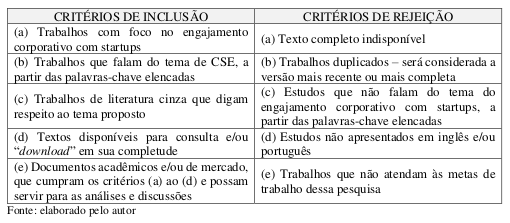
\includegraphics[]{Quadros/quadro-exemplo}}
  \source{Elaborado pelo autor}
  \label{quadro-exemplo}
\end{quadro}

And taking advantage of the quote from Satoshi Nakamoto, there are also those who say: "Bitcoin was not supposed to be like that. This is not what Satoshi Nakamoto conceived". Note, I don't know what exactly the individual or group behind the Bitcoin invention conceived. But you see, every human invention encapsulates the knowledge and knowhow of its creator. Encapsulate your ideas. But after "free in the world", invention has a "life of its own", and the ecosystem that was created from the invention has a life of its own. For good and for bad. There is not much more to be said for this.

We are near the end of the opinions I would like to express. One of the last concerns the opinions of politicians, investors, bankers and researchers about the future potential for cryptocurrencies. As I've already expressed, I see no reason to treat cryptocurrencies as an innovation unlike any other technological advance seen in humanity. And so, I am optimistic about the potential of cryptocurrencies, but realistic, far from the detachment from reality of some "moon boys". Now, one of the nuisances driving the perceived value of cryptocurrencies up is good news coming from these industries, which is fair, because it implies progress in adoption. On the other hand, there is the impact of bad news also coming from politicians, investors, bankers and researchers. And it is on this news that I want to do one of our latest mental exercises.

These people, sometimes representatives of large organizations, are ultimately the guardians of the status quo, for better or for worse. The opinions they declare, therefore, never define the true disruptive potential of cryptocurrencies, but rather the position that public opinion is wanted to believe on the subject. What do you expect to hear, for example, in an interview with, for example, an FED director? Do you think it's possible that he'll say something like: "Cryptocurrencies are indeed disruptive, they have enormous potential to transform the current financial system, and it's all a shame, because the organization I represent tends to lose more and more relevance because of it. of that and we will also lose the monopoly of issuing fiat money". Do you really think that a representative of the status quo, public or private, will say something like this?

Representatives of the status quo will always present opinions in defense of the status quo. It doesn't matter which arguments are used. The arguments will sometimes be good, sometimes bad, but the purpose behind is always to maintain the status quo. Simultaneously with any attempt to maintain the status quo, there are organizations that perceive change as an opportunity to uplift the current status quo, that is, to turn innovation into a competitive differential for themselves. These organizations can be companies or even countries, and in the case of cryptocurrencies, they can see: "Ok, I'm going to dive into cryptocurrencies, because I can make this a competitive advantage for my country."

It is a natural scenario, inherent to any major transformation in society, markets, form and type of goods and services provided. The point is: bullish news about crypto adoption is indeed bullish news. But you have to be careful with pessimistic news, because deep down, from the beginning, you never expected anything different after all. Organizations that find themselves in a position of dominance of the current status quo, in control of the financial system, will only take positive moves in favor of cryptocurrencies to avoid a "greater evil" from falling behind in relation to other organizations that adopt cryptos as a competitive differential.

And as a last reflection, I invite you to the following reflection: how wrong can all this go? Could it be that all the disruptive potential of cryptocurrencies hasn't already been priced in, and haven't we gone much further? This question is very pertinent. The most pertinent for the cryptocurrency investor after all. The "moon boys" want us to believe that "there are no limits", but in my opinion, there is a limit. Although the adoption of cryptos by society occurs extremely quickly and painlessly, without the need for a "war" against the current status quo, even if the entire world economic system is transformed, there are still limits to the intrinsic and extrinsic value of the sector. Remember the economy is bigger than that.

Judging by the innovations that cryptocurrencies are likely to bring, I believe there is still room for investment in the sector, without it being detached from the real potential of generating value to society. And I believe this because, a lot is said about cryptoCURRENCY, but beyond that, the central point here is not the money, but the transactions. And transactions aren't just economical. Every exchange of information in social dynamics is a transaction. The combination of cryptography with a decentralized consensus protocol undoubtedly finds its greatest utility in the financial system, but it is far from being the last. Ultimately, a decentralized consensus protocol is likely to change the dynamics of the entire internet as we know it today. This is definitely not a small thing, and it is definitely not of little value.

\begin{landscape}
  \begin{figure}[!hbt]
    \centering
    \caption{Uma figura deitado de exemplo}
    \makebox[0pt]{
\includegraphics[width=20cm,height=15cm]{Quadros/quadro-exemplo2}}
    \source{Elaborado pelo autor}
    \label{figura-exemplo2}
  \end{figure}
\end{landscape}

And taking advantage of the quote from Satoshi Nakamoto, there are also those who say: "Bitcoin was not supposed to be like that. This is not what Satoshi Nakamoto conceived". Note, I don't know what exactly the individual or group behind the Bitcoin invention conceived. But you see, every human invention encapsulates the knowledge and knowhow of its creator. Encapsulate your ideas. But after "free in the world", invention has a "life of its own", and the ecosystem that was created from the invention has a life of its own. For good and for bad. There is not much more to be said for this.

We are near the end of the opinions I would like to express. One of the last concerns the opinions of politicians, investors, bankers and researchers about the future potential for cryptocurrencies. As I've already expressed, I see no reason to treat cryptocurrencies as an innovation unlike any other technological advance seen in humanity. And so, I am optimistic about the potential of cryptocurrencies, but realistic, far from the detachment from reality of some "moon boys". Now, one of the nuisances driving the perceived value of cryptocurrencies up is good news coming from these industries, which is fair, because it implies progress in adoption. On the other hand, there is the impact of bad news also coming from politicians, investors, bankers and researchers. And it is on this news that I want to do one of our latest mental exercises.

These people, sometimes representatives of large organizations, are ultimately the guardians of the status quo, for better or for worse. The opinions they declare, therefore, never define the true disruptive potential of cryptocurrencies, but rather the position that public opinion is wanted to believe on the subject. What do you expect to hear, for example, in an interview with, for example, an FED director? Do you think it's possible that he'll say something like: "Cryptocurrencies are indeed disruptive, they have enormous potential to transform the current financial system, and it's all a shame, because the organization I represent tends to lose more and more relevance because of it. of that and we will also lose the monopoly of issuing fiat money". Do you really think that a representative of the status quo, public or private, will say something like this? \footnote{Este é um teste para checar o correto funcionamento das notas de rodapé.}

\begin{longtable}{| p{.20\textwidth} | p{.80\textwidth} |}
\hline
foo & bar \\ \hline
foo & bar \\ \hline
foo & bar \\ \hline
foo & bar \\ \hline
foo & bar \\ \hline
foo & bar \\ \hline
foo & bar \\ \hline
foo & bar \\ \hline
foo & bar \\ \hline
foo & bar \\ \hline
foo & bar \\ \hline
\caption{Your caption here} % needs to go inside longtable environment
\label{tab:myfirstlongtable}
\end{longtable}

Representatives of the status quo will always present opinions in defense of the status quo. It doesn't matter which arguments are used. The arguments will sometimes be good, sometimes bad, but the purpose behind is always to maintain the status quo. Simultaneously with any attempt to maintain the status quo, there are organizations that perceive change as an opportunity to uplift the current status quo, that is, to turn innovation into a competitive differential for themselves. These organizations can be companies or even countries, and in the case of cryptocurrencies, they can see: "Ok, I'm going to dive into cryptocurrencies, because I can make this a competitive advantage for my country."

It is a natural scenario, inherent to any major transformation in society, markets, form and type of goods and services provided. The point is: bullish news about crypto adoption is indeed bullish news. But you have to be careful with pessimistic news, because deep down, from the beginning, you never expected anything different after all. Organizations that find themselves in a position of dominance of the current status quo, in control of the financial system, will only take positive moves in favor of cryptocurrencies to avoid a "greater evil" from falling behind in relation to other organizations that adopt cryptos as a competitive differential.

And as a last reflection, I invite you to the following reflection: how wrong can all this go? Could it be that all the disruptive potential of cryptocurrencies hasn't already been priced in, and haven't we gone much further? This question is very pertinent. The most pertinent for the cryptocurrency investor after all. The "moon boys" want us to believe that "there are no limits", but in my opinion, there is a limit. Although the adoption of cryptos by society occurs extremely quickly and painlessly, without the need for a "war" against the current status quo, even if the entire world economic system is transformed, there are still limits to the intrinsic and extrinsic value of the sector. Remember the economy is bigger than that.

Judging by the innovations that cryptocurrencies are likely to bring, I believe there is still room for investment in the sector, without it being detached from the real potential of generating value to society. And I believe this because, a lot is said about cryptoCURRENCY, but beyond that, the central point here is not the money, but the transactions. And transactions aren't just economical. Every exchange of information in social dynamics is a transaction. The combination of cryptography with a decentralized consensus protocol undoubtedly finds its greatest utility in the financial system, but it is far from being the last. Ultimately, a decentralized consensus protocol is likely to change the dynamics of the entire internet as we know it today. This is definitely not a small thing, and it is definitely not of little value.
